\documentclass{article}
\usepackage[utf8]{inputenc}
\usepackage[T1]{fontenc}
\usepackage{graphicx}
\DeclareUnicodeCharacter{03B5}{\ensuremath{\varepsilon}}
\usepackage{hyperref}

% Kódování a česká lokalizace
\usepackage[utf8]{inputenc}
\usepackage[T1]{fontenc}
\usepackage[czech]{babel}

% Okraje stránky a typografie
\usepackage[margin=2.5cm]{geometry}
\usepackage{lmodern}
\usepackage{microtype}
\usepackage{parskip}


\title{Dokumentace projektu do IFJ}
\author{
  Dvořák, Štěpán\\
  xdvoras00\\
  id: 281757\\ \\
  Havránek, Kristián\\
  xhavrak00\\
  id: 281962
  \and
  Dohnal, Jiří\\
  xdohnaj00\\
  id: 282706\\ \\
  Zahradníček, Ivo\\
  xzahrai00\\
  id: 282396
  }
\begin{document}
\begin{figure}
    \centering
    
\includegraphics[width=0.5\textwidth]{fitlogo1_cz.pdf}
\end{figure}
\maketitle


\section{Obecné informace}
\large \href{https://github.com/stepadvo/IFJ-projekt}{odkaz na repozitář na GitHub}

\large Zvolená varianta: varianta vv-BVS
\subsection{Implementovaná rozšíření}
FUNEXP – funkce ve výrazech

BOOLTHEN – pravdivostní hodnoty

CONTROL – rozšířené řídicí struktury

\subsection{Rozdělení bodů}
Vzhledem k tomu, že nodošlo k žádným významným relativním nedostatkům v aktivitě jsme se rozhodli body rozdělit body přibližně rovnoměrně. Více bodů jsme přidělili Štěpánovi Dvořákovi za vedení týmu a pomoc s prací ostatním a Jiřímu dohnalovi za zpracování komplexnější a větší časti projektu (syntaktické analýzy).

Štěpán Dvořák - 27\%

Dohnal, Jiří - 25\%

Havránek, Kristián - 24\%

Zahradníček, Ivo - 24\%

\newpage
\section{Obecná architektura}

Spolupráce syntaktického a lexikálního analyzátoru se v našem projektu od standartního syntaxí řízeného překladu nijak neliší. Z důvodu kontroly návratových funkcí jsme se rozhodli, že sémantická analýza bude rekurzivně kontrolovat funkce, narazí-li na fuknci se zatím neznámým návratovým typem, proto syntaktické analýza nevolá sémantické akce a přímo volá nezkontrolované \texttt{AST} popisující celý zdrojový kód. Sémantická analýza poté zkontroluje celé \texttt{AST} a poté předává zkontrolovaný podstrom, reprezentující blok/funkci generátoru kódu.

\begin{figure}[h]
    \centering
    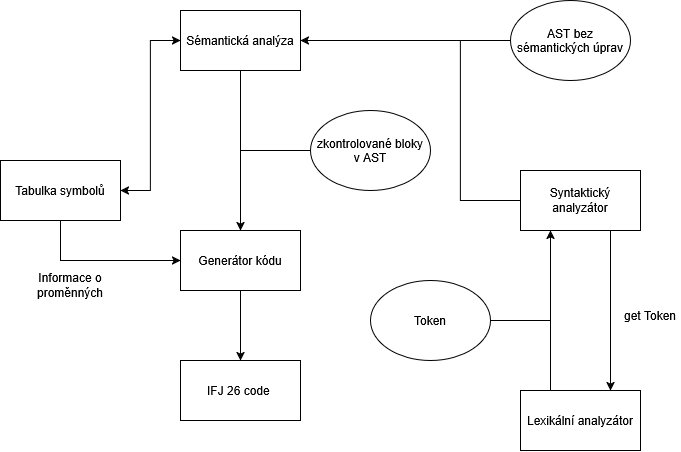
\includegraphics[width=1\textwidth]{diagram-blokové_schéma.png}
    \caption{Blokové schéma překladače}
\end{figure}
\newpage
\section{Práce v týmu}
- Meetingy jednou za týden
    1. část plánování struktury překladače
    2. část CODE reviews

- Případné shůzky "jeden na jednoho"
    1. procházení kódu co se neprošel na schůzkách

- Komunikace převážně přes Diskord

- Formátování
    1. Pojmenování proměnných a funkcí: camel case
    2. LLVM formátování pomocí clang-format

\subsection{Využití LLMs}
Umělou inteligenci jsme používali převážně pro generaci testů. Případně pro vysvětlení nedostatků, hledání chyb, v neposlední řadě pro případnou konzultaci kladů a záporů nápadů návrhů.

\section{Moduly programu}

- \texttt{token.c/.h} - Definuje strukturu Token.

- \texttt{lexer.c/.h} - Zajišťuje funkcionalitu lexikálního analyzátoru.

- \texttt{parser.c/.h} - Rekurzivním sestupem zpracovává syntax a sestavuje AST. Dále řídí i redukce výrazů.

- \texttt{expression.c/.h} - Poskytuje precedenční tabulku a zásobník pro syntaktickou analýzu výrazů.

- \texttt{ast.c/.h} - Definuje uzly AST a funkce pro jejich vytváření a uvolňování.

- \texttt{semantics.c/.h} - Základní funkce sémantické analýzy.

- \texttt{internalSemantics.c/.h} - Interní funkce sémantické analýzy.

- \texttt{builtins.c/.h} - Funkce připravující tabulku symbolů vložením vestavěných funkcí.

- \texttt{collectFunctionHeaders.c/.h} - Funkce vkládanící funkce programu do tabulky symbolů.

- \texttt{bst.h/.c} - Obsahuje abstraktní datový typ vv-BST (odděleno od tabulek symbolů pro lepší přehlednost kódu a případné použití do budoucna).

- \texttt{symtable.h/.c} - Obsahuje globální tabulku symbolů funkcí i lokální tabulky symbolů proměnných.

- \texttt{generator.h/.c} - Obsahuje generátor cílového kódu generující ze zkontrolovaných částí AST.

- \texttt{compiler.h/.c}, \texttt{errcode.c} - Obsahuje definice a funkce používané většínou modulů - vstupní funkce, hlášení chyb na standartní chybový výstup.


\newpage

\section{Lexikální analýza}
\subsection{Rozdělení modulů}

Soubory \texttt{lexer.c} a \texttt{lexer.h} zajišťují lexikální analýzu: čtení vstupního proudu, rozpoznávání tokenů a sledování jejich pozice. Hlavička zveřejňuje rozhraní lexeru, ale vnitřní struktura \texttt{Lexer} je definována pouze v implementaci.

Soubory \texttt{token.c} a \texttt{token.h} definují společnou reprezentaci tokenů pro lexer a parser. Obsahují výčet \texttt{TokenType}, atributy tokenů, informace o pozici a funkci \texttt{tokenFree()} pro uvolnění vlastněného textu.

\subsection{Komunikace s parserem}

Lexer se vytváří funkcí \texttt{lexerCreate()}, která dostává otevřený vstupní proud \texttt{FILE *}. Parser následně podle potřeby volá \code{getToken()} a získává vždy jeden další token. Celý vstup se tedy nemusí předem načíst do paměti.

Struktura \texttt{Token} obsahuje typ tokenu, jeho případný atribut, řádek a sloupec začátku a metadata pro zpracování logických řádků. Atribut je reprezentován unií\texttt{TokenAttribute}: může obsahovat celočíselnou, desetinnou nebo Boolean hodnotu či text identifikátoru a řetězce.

\subsection{Rozpoznávání lexémů}

Rozpoznávání je implementováno ručně pomocí větvení podle prvního znaku a pomocných funkcí pro jednotlivé skupiny lexémů. Stavy rozpoznávání jsou vyjádřeny tokem programu, smyčkami a příznaky.

Identifikátor se nejprve načte celý. Funkce \texttt{lexerIdentifierType()} ho potom porovná s tabulkou klíčových slov, která zahrnuje také Boolean literály \texttt{true} a \texttt{false}.

Číselné literály zpracovává \texttt{lexerReadNumber()}. Postupně rozpoznává číslice, podtržítkové oddělovače, případnou desetinnou část, exponent a příponu d nebo D u \texttt{Double}. Podtržítka se do převáděného textu neukládají. Výsledná hodnota vzniká pomocí \texttt{strtoll()} nebo \texttt{strtod()}. Současná implementace podle týmové dohody odmítá také zápisy. 01.5 a 01e2.

Platný číselný token ukončíme před znakem následujícího tokenu. Například 10abc vrátí číslo 10 a identifikátor \texttt{abc}; přípustnost jejich posloupnosti posoudí parser.

Obyčejné řetězce vyhodnocují podporované escape sekvence. Víceřádkové řetězce ohraničené třemi uvozovkami uchovávají obsah doslova, včetně odřádkování.

\subsection{Pomocný stav nad rámec konečného automatu}

Vnořené blokové komentáře se zpracovávají pomocí čítače \texttt{depth}. Začátek dalšího komentáře čítač zvýší a uzavírací dvojice jej sníží. Komentář končí při návratu na nulu.

Čítač \texttt{parenDepth} sleduje otevřené kulaté závorky a umožňuje rozlišovat odřádkování uvnitř a vně závorek. Další pomocné údaje uchovávají odsazení a stav fyzického a logického řádku.

Nahlížení na následující znak zajišťuje \texttt{lexerPeekChar()}. Pomocný buffer \texttt{pendingCharacter} se využívá například při rozlišení desetinné tečky od samostatné tečky v zápisu \texttt{42.toString}.

\subsection{Řádky a odsazení}

Lexer rozlišuje fyzické a logické řádky. Neprázdný logický řádek mimo závorky ukončuje tokenem \texttt{TOKEN\_NEWLINE}. Prázdné a komentářové řádky přeskakuje.

První skutečný token logického řádku označuje příznakem \texttt{startsLogicalLine} a přidává počet úvodních mezer do \texttt{indent}. Příznak \texttt{newlineBefore} zaznamenává odřádkování před tokenem, včetně případů, kdy uvnitř závorek nevzniká samostatný token nového řádku.

Lexer odmítá tabulátor v odsazení neprázdného řádku a kontroluje větší odsazení pokračování uvnitř závorek. Otevírání a ukončování bloků podle odsazení řeší parser, který zná syntaktický kontext. Na konci souboru lexer případně doplní ukončení posledního logického řádku.

\subsection{Správa paměti a chyby}

Identifikátory a řetězce používají dynamické buffery, jejichž kapacita se při zaplnění zvětšuje na dvojnásobek. Výsledný text vlastní token.

Funkce \texttt{tokenFree()} uvolní textový atribut a vynuluje token. \texttt{getToken()} ji při opětovném použití stejného výstupního tokenu zavolá před načtením nového obsahu. Zničení lexeru neuvolňuje již vrácené tokeny ani neuzavírá vstupní proud.

Chyby se oznamují společnou funkcí \texttt{logErr()}. Lexer vrací \texttt{LEXER\_ERROR} pro lexikální chyby a \texttt{LEXER\_INTERNAL\_ERROR} například při selhání alokace nebo čtení. Sám program neukončuje a nepřepisuje již zaznamenaný nenulový globální chybový kód.

\subsection{Testování}

Pro lexer je připraveno deset testů a pro tokeny tři testy ve frameworku GoogleTest. Spouštějí se příkazem \texttt{make test}, který zajistí také překlad potřebných modulů.

Testy pokrývají typy tokenů, hodnoty literálů, hranice čísel, řetězce, komentáře, pozice, odsazení, chybné vstupy a chování na konci souboru. Ověřují také nezávislé vlastnictví textu, opakované uvolňování tokenů a zachování prvního chybového kódu. Poslední změna doplnila pět případů pro rozdělení navazujícího čísla a identifikátoru.

\newpage
\subsection{Deterministický konečný automat}
\begin{figure}[ht]
    \centering
    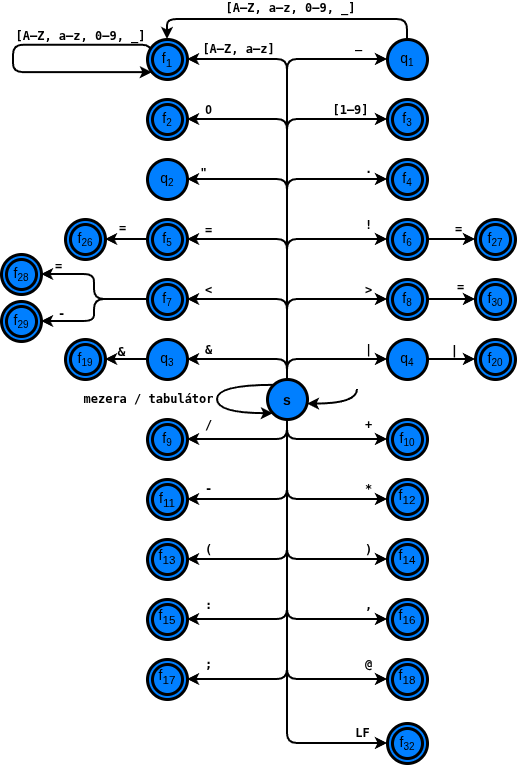
\includegraphics[width=0.6\textwidth]{dka.png}
    \caption{Obecná podoba DKA}
\end{figure}
\begin{figure}[ht]
    \centering
    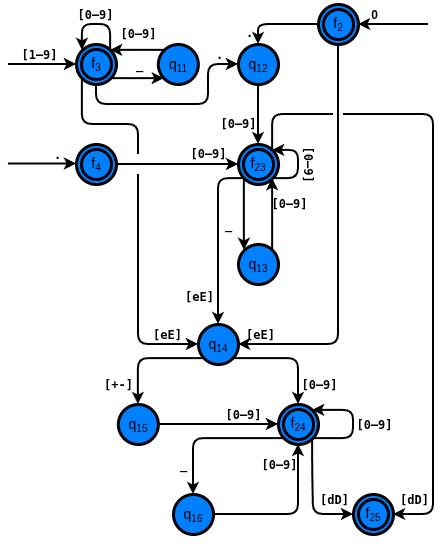
\includegraphics[width=0.7\textwidth]{cisla.png}
    \caption{přiblížení DKA pro zpracování číselných literálů}
\end{figure}
\begin{figure}[ht]
    \centering
    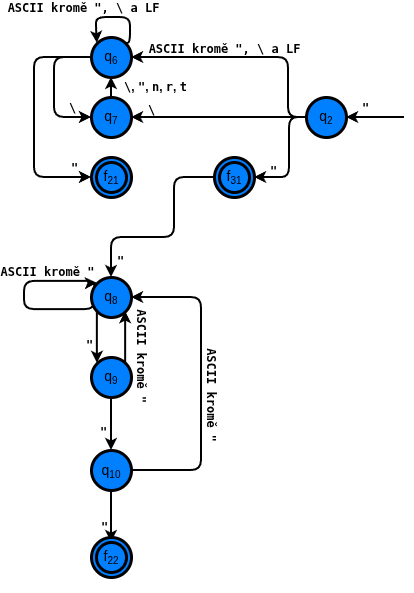
\includegraphics[width=0.7\textwidth]{retezce.png}
    \caption{přiblížení DKA pro zpracování řetězcových literálů}
\end{figure}
\begin{figure}[ht]
    \centering
    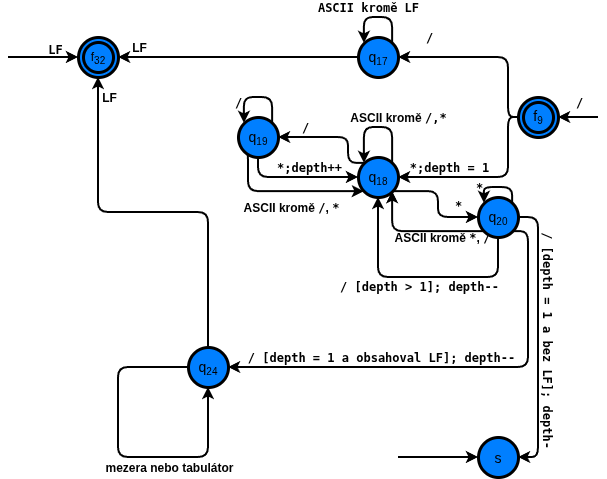
\includegraphics[width=0.9\textwidth]{komentare.png}
    \caption{přiblížení DKA pro zpracování komentářů}
\end{figure}

\clearpage
\section{Syntaktická analýza}

Syntaktický analyzátor používá rekurzivní sestup. Výrazy zpracovává samostatnou precedenční analýzou.

Parser prochází tokeny a podle začátku konstrukce volí funkci. U bloků kontroluje odsazení pomocí atributů tokenů.

\subsection{LL gramatika}

1. \textless program\textgreater{} → \textless prolog\textgreater{} \textless function-list\textgreater{} EOF

2. \textless prolog\textgreater{} → import id(ifj26) . * NL

3. \textless function-list\textgreater{} → \textless function\textgreater{} \textless function-list\textgreater{}

4. \textless function-list\textgreater{} → ε

5. \textless function\textgreater{} → \textless annotation\textgreater{} def id ( \textless parameters\textgreater{} ) \textless return-type\textgreater{} = \textless function-body\textgreater{}

6. \textless annotation\textgreater{} → @ id(main) \textless annotation-end\textgreater{}

7. \textless annotation\textgreater{} → ε

8. \textless annotation-end\textgreater{} → NL

9. \textless annotation-end\textgreater{} → ε

10. \textless parameters\textgreater{} → \textless parameter\textgreater{} \textless remaining-parameters\textgreater{}

11. \textless parameters\textgreater{} → ε

12. \textless parameter\textgreater{} → id : \textless type\textgreater{}

13. \textless remaining-parameters\textgreater{} → , \textless parameter-after-comma\textgreater{}

14. \textless remaining-parameters\textgreater{} → ε

15. \textless parameter-after-comma\textgreater{} → \textless parameter\textgreater{} \textless remaining-parameters\textgreater{}

16. \textless parameter-after-comma\textgreater{} → ε

17. \textless return-type\textgreater{} → : \textless type\textgreater{}

18. \textless return-type\textgreater{} → ε

19. \textless type\textgreater{} → Int

20. \textless type\textgreater{} → Double

21. \textless type\textgreater{} → String

22. \textless type\textgreater{} → Boolean

23. \textless type\textgreater{} → Unit

24. \textless function-body\textgreater{} → NL \textless block\textgreater{}

25. \textless function-body\textgreater{} → FE

26. \textless block\textgreater{} → IN \textless statement\textgreater{} \textless block-continuation\textgreater{} OUT

27. \textless block-continuation\textgreater{} → ; \textless statement\textgreater{} \textless block-continuation\textgreater{}

28. \textless block-continuation\textgreater{} → NL \textless after-newline\textgreater{}

29. \textless block-continuation\textgreater{} → NEXT \textless statement\textgreater{} \textless block-continuation\textgreater{}

30. \textless block-continuation\textgreater{} → ε

31. \textless after-newline\textgreater{} → \textless statement\textgreater{} \textless block-continuation\textgreater{}

32. \textless after-newline\textgreater{} → ε

33. \textless statement\textgreater{} → val \textless variable-declaration\textgreater{}

34. \textless statement\textgreater{} → var \textless variable-declaration\textgreater{}

35. \textless statement\textgreater{} → return \textless return-value\textgreater{}

36. \textless statement\textgreater{} → \textless if-statement\textgreater{}

37. \textless statement\textgreater{} → \textless while-statement\textgreater{}

38. \textless statement\textgreater{} → \textless for-statement\textgreater{}

39. \textless statement\textgreater{} → id \textless identifier-continuation\textgreater{}

40. \textless statement\textgreater{} → E\_OTHER

41. \textless variable-declaration\textgreater{} → id \textless optional-type\textgreater{} = E

42. \textless optional-type\textgreater{} → : \textless type\textgreater{}

43. \textless optional-type\textgreater{} → ε

44. \textless return-value\textgreater{} → E

45. \textless return-value\textgreater{} → ε

46. \textless identifier-continuation\textgreater{} → = E

47. \textless identifier-continuation\textgreater{} → E\_CONT

48. \textless if-statement\textgreater{} → if E then \textless if-body\textgreater{} \textless optional-else\textgreater{}

49. \textless if-body\textgreater{} → NL \textless block\textgreater{}

50. \textless if-body\textgreater{} → INLINE\_IF

51. \textless optional-else\textgreater{} → else \textless else-body\textgreater{}

52. \textless optional-else\textgreater{} → ε

53. \textless else-body\textgreater{} → \textless if-statement\textgreater{}

54. \textless else-body\textgreater{} → NL \textless block\textgreater{}

55. \textless else-body\textgreater{} → INLINE\_NONIF

56. \textless while-statement\textgreater{} → while E do \textless body\textgreater{}

57. \textless body\textgreater{} → NL \textless block\textgreater{}

58. \textless body\textgreater{} → INLINE\_STMT

59. \textless for-statement\textgreater{} → for \textless for-header\textgreater{}

60. \textless for-header\textgreater{} → \textless generator\textgreater{} \textless guards\textgreater{} do \textless body\textgreater{}

61. \textless for-header\textgreater{} → NL \textless generator\textgreater{} NL \textless multiline-guards\textgreater{} do \textless body\textgreater{}

62. \textless generator\textgreater{} → id \textless- E \textless range-specification\textgreater{}

63. \textless range-specification\textgreater{} → id(to) E \textless optional-step\textgreater{}

64. \textless range-specification\textgreater{} → id(until) E

65. \textless optional-step\textgreater{} → id(by) E

66. \textless optional-step\textgreater{} → ε

67. \textless guards\textgreater{} → if E \textless guards\textgreater{}

68. \textless guards\textgreater{} → ε

69. \textless multiline-guards\textgreater{} → if E NL \textless multiline-guards\textgreater{}

70. \textless multiline-guards\textgreater{} → ε

71. \textless function-call\textgreater{} → id ( \textless arguments\textgreater{} )

72. \textless arguments\textgreater{} → E \textless remaining-arguments\textgreater{}

73. \textless arguments\textgreater{} → ε

74. \textless remaining-arguments\textgreater{} → , \textless argument-after-comma\textgreater{}

75. \textless remaining-arguments\textgreater{} → ε

76. \textless argument-after-comma\textgreater{} → E \textless remaining-arguments\textgreater{}

77. \textless argument-after-comma\textgreater{} → ε

\newpage
\subsubsection{Použité symboly}

E -- část programu předaná precedenční analýze, která z ní vytvoří uzel AST

E\_OTHER -- výraz nezačínající identifikátorem ani klíčovým slovem příkazu

E\_CONT -- pokračování výrazu po identifikátoru, který už parser načetl

FE -- výraz tvořící jednořádkové tělo funkce, ukončený koncem řádku nebo EOF

NL -- konec logického řádku

IN -- vstup do více odsazeného bloku

OUT -- návrat do nadřazeného bloku

NEXT -- další příkaz po již zpracovaném vnořeném bloku

INLINE\_IF -- jednořádkové tělo za then, pokud nenásleduje NL

INLINE\_NONIF -- jednořádkové tělo za else, které nezačíná dalším if

INLINE\_STMT -- jednořádkové tělo cyklu za do, pokud nenásleduje NL

id(slovo) -- identifikátor s daným textem

ε -- prázdný řetězec

Pomocné značky pro odsazení a jednořádková těla nejsou tokeny lexeru.

Slova main, ifj26, to, until a by se kontrolují podle textu identifikátoru.

Koncová čárka v parametrech a argumentech je možná jen při zalomení před ). Výrazové if vyžaduje else, u příkazového if je nepovinné. by lze použít jen s to.

U prázdného return se výraz nečte před NL, ;, EOF a v odpovídajícím kontextu i před else. U víceřádkového for se kontroluje odsazení generátoru, stráží a do.

\subsubsection{Předávání výrazů}

Při začátku příkazu identifikátorem parser nejdříve rozliší přiřazení od výrazu. Funkce parseIdentifierValue() pak rozliší proměnnou od volání. Zbytek výrazu zpracuje parseExpressionFromValue().

ExpressionStops určuje, před kterými symboly výraz skončí, např. před else, to, until, by nebo if ve for. Pravidla 71--77 popisují volání, která se zpracovávají uvnitř výrazů.
\newpage

\subsection{LL tabulka}

Tyto tabulky jsou části jedné LL tabulky. Čísla odkazují na pravidla výše, pomlčka znamená chybu. Pomocné značky popisují rozhodování parseru. Nejde o úplnou LL(1) tabulku nad tokeny lexeru.

\begin{figure}[ht]
    \centering
    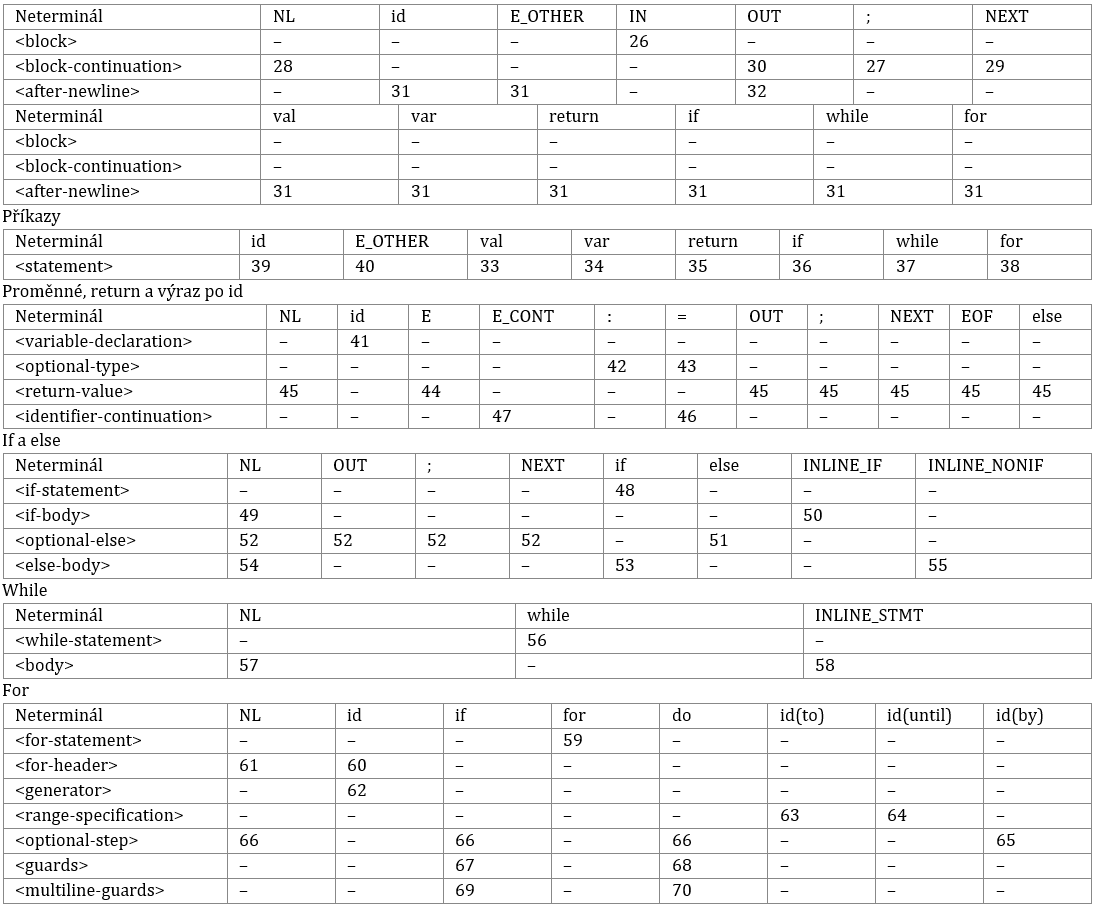
\includegraphics[width=1\textwidth]{obrazek.png}
    \caption{LL tabulka 1.část}
\end{figure}
\begin{figure}[ht]
    \centering
    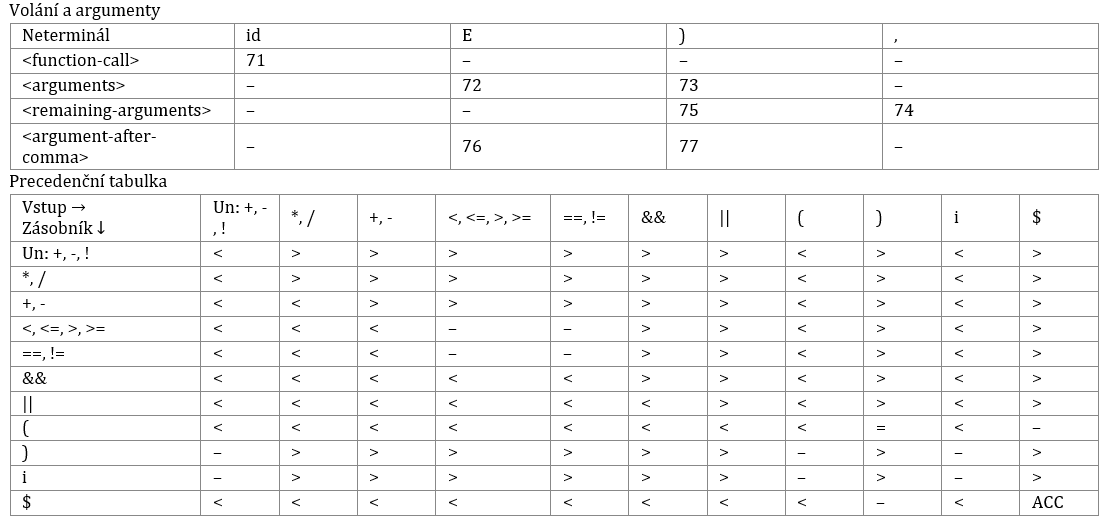
\includegraphics[width=1\textwidth]{obrazek3.png}
    \caption{LL tabulka 2.část}
\end{figure}
\newpage
\begin{figure}[ht]
    \centering
    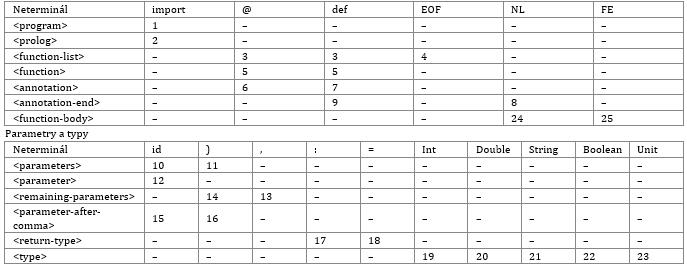
\includegraphics[width=1\textwidth]{obrazek2.png}
    \caption{LL tabulka 3.část}
\end{figure}
Řádky: symbol na zásobníku

Sloupce: vstupní symbol

Vztahy:

\textless{} - přesun

\textgreater{} - redukce

= - zpracování závorek

ACC - přijetí

-- - chyba

i -- hodnota (literál, identifikátor, výsledek volání nebo výrazový if)

\$ -- začátek a konec analyzovaného výrazu

\subsection{Výrazy}

Výrazy jsou zpracovávány operátorovou precedenční analýzou metodou shift-reduce. Precedenční tabulka určuje, kdy se na zásobník přidá další symbol a kdy se provede redukce.

Při redukci se podle symbolů na vrcholu zásobníku vytvářejí uzly AST pro hodnoty a unární nebo binární operace. Prázdné závorky () se zpracují jako literál typu Unit. Začátek redukované části se zvlášť neoznačuje.

\subsection{Tvorba AST}

Kořenem AST je program se seznamem funkcí. Každá funkce má tělo jako blok se seznamem příkazů. Údaje různých druhů uzlů jsou uloženy v union data. Výrazy se skládají do uzlů pro operátory, literály, identifikátory a volání funkcí.

Jednořádkové tělo se také ukládá jako blok s jedním příkazem. Funkce parse() vrací hotový strom pro další analýzu. freeAst() jeho uzly rekurzivně uvolňuje.

\newpage
\section{Sémantická analýza}
\subsection{překladač -> sémantika}
překladač bere \texttt{AST} od parseru a volá \texttt{semanticAnalyze}, z něj dostává ERRCODE. V \texttt{semantics.c}, které bere AST a vytváří \texttt{symtable}, stav generátoru a \texttt{SemCtx}, na konci rohoduje o výstupu, hlásí chybu 99 při selhání inicializace.
\subsection{pomocné moduly \texttt{builtins.h/.c} a \texttt{collectFunctionHeaders.h/.c}}
\texttt{builtins.c} si z \texttt{SemCtx} bere vlastní tabuilku \texttt{BuiltinDef}, volá záznami vestavěných funcí do globální tabulky funkcí, hlásí 99 při nezdařené inicializaci. \texttt{CollectFunctionHeaders.c/} bere si seznam \texttt{$AST\_FUNC\_DEF$} z kořene a volá záznamy funkcí v tabulce, stejně jako builtins hlasí 99, dále však i 3/4/5/6
\subsection{\texttt{internalSemantics.c}}
Hlavní funkcí v \texttt{internalSemantics.c} je \texttt{analyze funkction}, jejihž hlavním rolemi je příprava prostředí, kontrola návratového typu a generování těla. \texttt{analyzeBlock, analyzeStatement, analyzeVarDef, analyzeAssign, analyzeIf, analyzeWhile, analyzeFor, analyzeReturn} slouží jako pravidla pro jednotlivé kontrukce, \texttt{analyzeExpr} hlídá návratové typy výrazů, popř převadí typy např.: převádění \texttt{INT} na \texttt{DOUBLE} při provádění základních operací mezi \texttt{INT} a \texttt{DOUBLE}, vrámci \texttt{internalSemantics.c} jsou také pomocné \texttt{isCompatible, isNumeric, wrapInt2Double, findFuncIndex, endReturn}, které se strarají o neustále se opakující kontroly, např.: \texttt{is Compatible} kontroluje kompatibilitu dvou typů pro \texttt{analyzeExpr}.
\newpage

\section{Generátor cílového kódu}

Každý symbol funkce v globální tabulce symbolů obsahuje lokální tabulku symbolů, která ukládá pouze proměnné dostupné v současně analyzovaném/generovaném bloku. Je možné mít uloženo symboly proměnné do více lokálních tabulek v jednu chvíli. Symboly jsou ukládány do dynamického pole a do \texttt{vv-BST} se ukládají pouze indexy symbolu v těchto polích. To v zájmu rychlejšího vyprázdnění tabulek (změny kapacity pole), jednoduššího rozdělení podle rozsahů platnosti (blok ve zdrojovém kódu je rozsahem mezi 2 indexama v poli) a jednoduššího maskování (symbol zůstává v poli a nahradí se pouze jeho index ve \texttt{vv-BST}). Vzhledem k tomu, že tabulky nejsou schopné uložit proměnné napříč celým kódem, tak musí moduly pracující s nimi (sémantická analýza a generátor cílového kódy) pracovat současně.

Protože sémantická analýza zkontrolovala vše, co se má generovat, tak generátor cílového kódu předpokládá, že v ast odpovídá symbolům uloženým v tabulce symbolů a že je zkontrolovaná část generovatelná.
Pro zájmy testování je možné nechat generátor kódu, aby kontroloval správný stav tabulky symbolů definováním \texttt{IFJ\_GEN\_DEBUG}
Kód se generuje po blocích od listů ast ke kořeni, jak jej sémantická analýza zkontroluje.
Jelikoz semanticka analyza muze mit rozpracovanych nekolik funkci v ast v jeden moment, tak generátor umožňuje generovat kód do datových struktur, ve kterých se vygenerované bloky vkládají na svá místa do nadřazených bloků.
Po generaci všech bloků náležících funkci, přesune se jejich obsah do souvislého textu.
Aby se na standartní výstup vypsal cílový kód pouze v moment, kdy nebyla nalezena žádná chyba ve zdrojovém kódu se po dokončení sémantické analýzy rozhodne, jestli se výsledný kód vypíše nebo zahodí.


\end{document}
